\documentclass[tikz,border=4pt,11pt]{standalone}
\usepackage{amsmath}
\usetikzlibrary{arrows.meta}
\definecolor{ink}{RGB}{42,52,64}
\definecolor{first}{RGB}{146,79,26}
\definecolor{second}{RGB}{26,99,111}

% The four acyclic orientations of the path 1-2-3. Ascending edges (directed
% from the smaller to the larger label) are drawn thick in the first colour,
% sinks (vertices without outgoing edges) are circled in the second colour.
% Each orientation is labelled by (asc, sink) and its weight q^asc t^sink:
% (0,1) t, (1,1) q t, (1,2) q t^2, (2,1) q^2 t.

\begin{document}
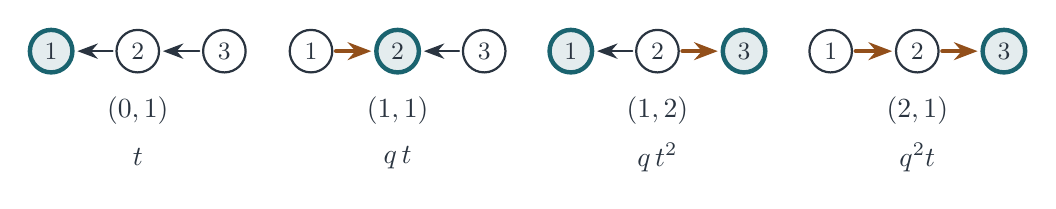
\begin{tikzpicture}[text=ink,line cap=round,x=1.1cm,y=1cm,
  vtx/.style={circle,draw=ink,fill=white,line width=.8pt,inner sep=0pt,
    minimum size=5.4mm,font=\small},
  sink/.style={vtx,draw=second,fill=second!12,line width=1.6pt},
  desc/.style={-{Stealth[length=2.6mm]},ink,line width=.8pt,shorten <=1pt,shorten >=1pt},
  asc/.style={-{Stealth[length=3mm]},first,line width=1.6pt,shorten <=1pt,shorten >=1pt}]

% (0,1): 2->1, 3->2
\begin{scope}[shift={(0,0)}]
  \node[sink] (a) at (0,0) {$1$};
  \node[vtx]  (b) at (1,0) {$2$};
  \node[vtx]  (c) at (2,0) {$3$};
  \draw[desc] (b) -- (a);
  \draw[desc] (c) -- (b);
  \node at (1,-.75) {$(0,1)$};
  \node at (1,-1.35) {$t$};
\end{scope}

% (1,1): 1->2, 3->2
\begin{scope}[shift={(3,0)}]
  \node[vtx]  (a) at (0,0) {$1$};
  \node[sink] (b) at (1,0) {$2$};
  \node[vtx]  (c) at (2,0) {$3$};
  \draw[asc]  (a) -- (b);
  \draw[desc] (c) -- (b);
  \node at (1,-.75) {$(1,1)$};
  \node at (1,-1.35) {$q\,t$};
\end{scope}

% (1,2): 2->1, 2->3
\begin{scope}[shift={(6,0)}]
  \node[sink] (a) at (0,0) {$1$};
  \node[vtx]  (b) at (1,0) {$2$};
  \node[sink] (c) at (2,0) {$3$};
  \draw[desc] (b) -- (a);
  \draw[asc]  (b) -- (c);
  \node at (1,-.75) {$(1,2)$};
  \node at (1,-1.35) {$q\,t^2$};
\end{scope}

% (2,1): 1->2, 2->3
\begin{scope}[shift={(9,0)}]
  \node[vtx]  (a) at (0,0) {$1$};
  \node[vtx]  (b) at (1,0) {$2$};
  \node[sink] (c) at (2,0) {$3$};
  \draw[asc]  (a) -- (b);
  \draw[asc]  (b) -- (c);
  \node at (1,-.75) {$(2,1)$};
  \node at (1,-1.35) {$q^2t$};
\end{scope}
\end{tikzpicture}
\end{document}
